%==============================================================================
% experimental-setup.tex
%==============================================================================

\part{Appendices}
\label{part:appendices}

\chapter{Experimental Setup}
\label{chap:experimental-setup}

The performance results were obtained on two different machines, an
Intel Core2 Duo and an Intel Nehalem system.

\section{Intel Core2 Duo}
\label{sec:experimental-setup-marvin}

The machine has one Intel Core2 Duo Processor T9550 with two cores and
4 GB RAM. Each core has its separate level 1 cache and the 6 MB level
2 cache is shared between the two cores (Figure
\ref{fig:experimental-setup-marvin}).

\begin{figure}[htb]
  \centering
  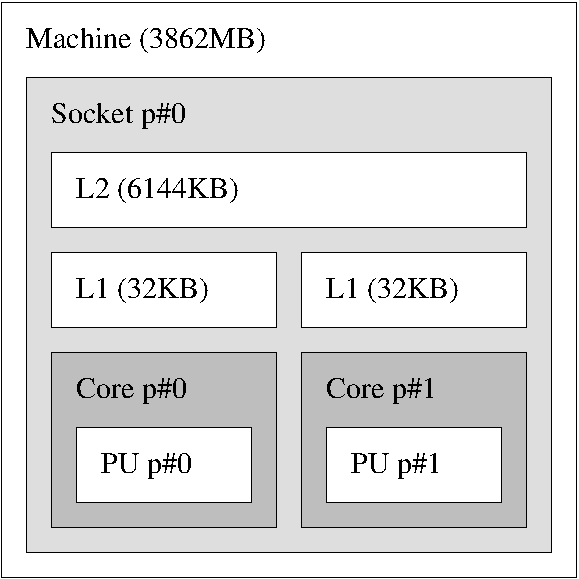
\includegraphics[width=0.59\textwidth]{experimental-setup/marvin}
  \caption{Intel Core2 Duo}
  \label{fig:experimental-setup-marvin}
\end{figure}

The system runs Ubuntu 10.04 64-bit with kernel 2.6.32 and the JVM
used is Sun Hotspot JDK 1.6.0\_20.

\section{Intel Nehalem}
\label{sec:experimental-setup-mafushi}

This system includes two Intel Xeon E5520 quad-core processors based
on the Intel Nehalem micro architecture. The machine has 12 GB RAM and
each processor has a direct connection to half of the memory space via
an integrated memory controller (Figure
\ref{fig:experimental-setup-mafushi}). Additionally, each processor
has two QuickPath Interconnect interfaces \cite{Maddox2009}, one
connecting to the remote processor and one to the Input/Output hub.

While every core has its separate level 1 and level 2 caches, the
per-processor 8 MB level 3 cache is shared between all cores of the
same processor. The level 3 cache and the memory controllers of a
processor are considered to be a separate subsystem and the Intel
documentation refers to this subsystem as the \emph{uncore}.

We sometimes refer to a processor as a node to emphasize its
participation in forming a (large-scale) parallel system.

\begin{figure}[htb]
  \centering
  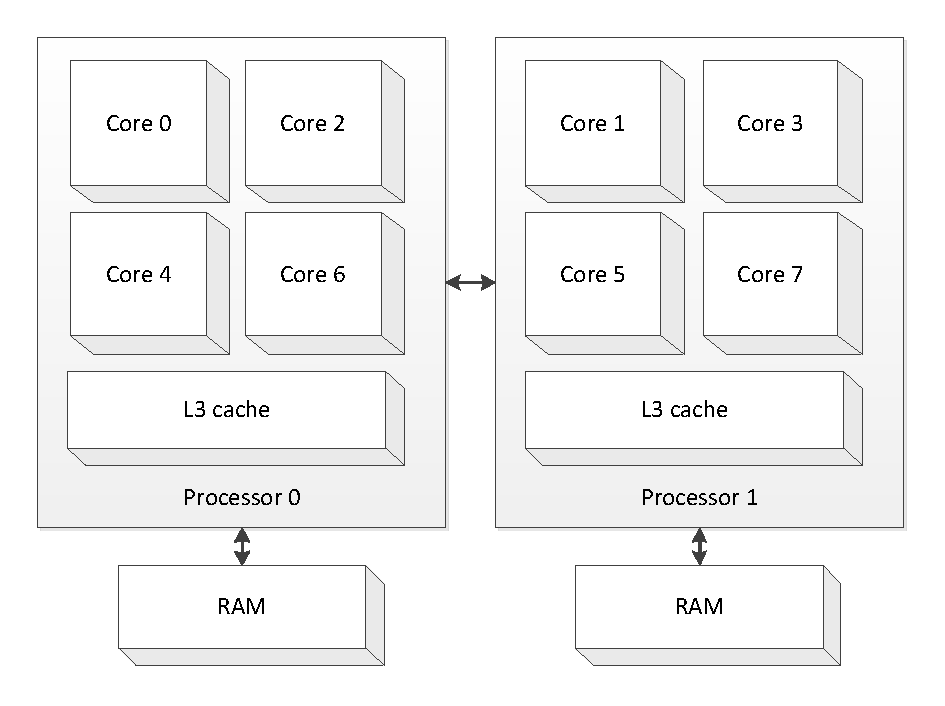
\includegraphics[width=0.61\textwidth]{experimental-setup/mafushi}
  \caption{Intel Nehalem in a two-processor configuration}
  \label{fig:experimental-setup-mafushi}
\end{figure}

The system runs Ubuntu 9.04 64-bit with kernel 2.6.29 patched to
support perfmon2 \cite{Eranian2008} and the JVM used is Sun Hotspot
JDK 1.6.0\_20.


%%% Local Variables: 
%%% mode: latex
%%% TeX-master: "thesis"
%%% End: 
